
\section{Virtual phase correction}

After finding the right shape, we still have to consider a last calibration parameter: the phase.
The discussion here will be around the CZ since it presents some more problems in respect to the iSWAP, but as always everything is more or less interchangeable.

\begin{figure}[ht]
    \centering
    \makebox[\textwidth][c]{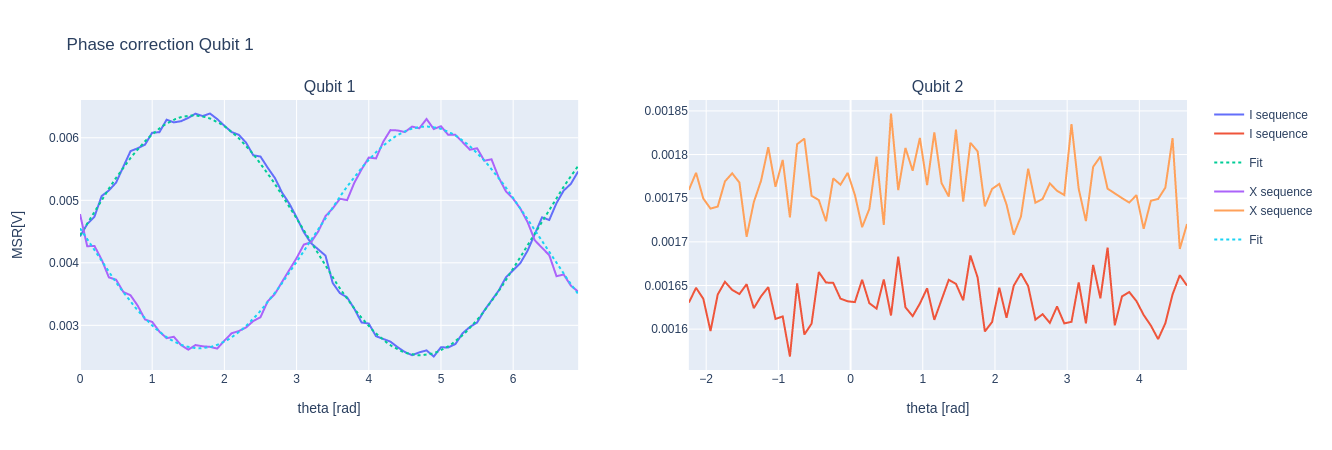
\includegraphics[width=1.3\textwidth]{Two-qubits calibration/Figures/phase_correction_1.png}}\\
    \makebox[\textwidth][c]{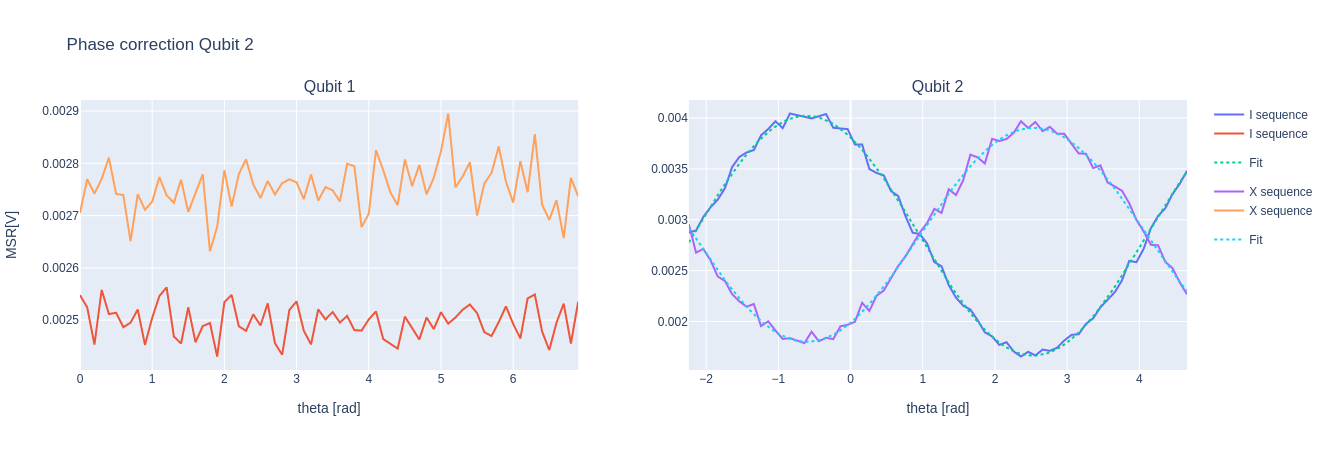
\includegraphics[width=1.3\textwidth]{Two-qubits calibration/Figures/phase_correction_2.png}}
    \caption{Calibrated virtual phase correction plot.}
    \label{fig:virtualphase}
\end{figure}

The problem is that so far we have ignored the role of the single-qubit phases acquired by tuning the qubit frequency (caused by simple time evolution). 
So, effectively we never implemented a CZ (or a iSWAP) but a CZ with the addition of a spurious relative phase between the qubits.
Critically, this phase is not dependent on the state of the control qubit, but is constant in all cases, so it will be fairly easy to implement a virtual correction once calibrated (so consider the presence of this phase for all successive pulses and measurements).

The experiment we perform is the following:
\begin{itemize}
    \item we initialize the system performing a $Y90$ pulse on the low frequency qubit and either a $I$ or a $X$ gate on the high frequency one;
    \item we apply the flux pulse for the two-qubit interaction;
    \item we undo the initial rotation on the high frequency qubit, by applying $I$ or $X$ again;
    \item we apply a $\Theta(90)$ pulse, so a rotation of $90^\circ$ around a certain angle $\theta$;
    \item we measure the two qubits;
    \item we repeat the measurement for multiple angles and for both $I$ and $X$ initial states.
\end{itemize}

Ideally, the high frequency qubit should not be affected at all by the gate, eventually some leakage to the $\ket 2$ state can be visible.

For the low frequency qubit, we should see, depending on the initial state of the control qubit, two different sinusoidal with a $90^\circ$ phase difference.
What we will actually see is presented in \cref{fig:virtualphase}.

The phase difference is not $90^\circ$ as expected but $(90+\epsilon)^\circ$ with $\epsilon$ being the virtual phase to consider for later sequences and measurements.












